\documentclass[12pt,]{book}
\usepackage{lmodern}
\usepackage{setspace}
\setstretch{1}
\usepackage{amssymb,amsmath}
\usepackage{ifxetex,ifluatex}
\usepackage{fixltx2e} % provides \textsubscript
\ifnum 0\ifxetex 1\fi\ifluatex 1\fi=0 % if pdftex
  \usepackage[T1]{fontenc}
  \usepackage[utf8]{inputenc}
\else % if luatex or xelatex
  \ifxetex
    \usepackage{mathspec}
  \else
    \usepackage{fontspec}
  \fi
  \defaultfontfeatures{Ligatures=TeX,Scale=MatchLowercase}
    \setmainfont[]{Montserrat}
\fi
% use upquote if available, for straight quotes in verbatim environments
\IfFileExists{upquote.sty}{\usepackage{upquote}}{}
% use microtype if available
\IfFileExists{microtype.sty}{%
\usepackage{microtype}
\UseMicrotypeSet[protrusion]{basicmath} % disable protrusion for tt fonts
}{}
\usepackage[marginpar=2cm, top=3cm, bottom=4cm]{geometry}
\usepackage{hyperref}
\hypersetup{unicode=true,
            pdfborder={0 0 0},
            breaklinks=true}
\urlstyle{same}  % don't use monospace font for urls
\usepackage[numbers]{natbib}
\bibliographystyle{plainnat}
\usepackage{longtable,booktabs}
\usepackage{graphicx,grffile}
\makeatletter
\def\maxwidth{\ifdim\Gin@nat@width>\linewidth\linewidth\else\Gin@nat@width\fi}
\def\maxheight{\ifdim\Gin@nat@height>\textheight\textheight\else\Gin@nat@height\fi}
\makeatother
% Scale images if necessary, so that they will not overflow the page
% margins by default, and it is still possible to overwrite the defaults
% using explicit options in \includegraphics[width, height, ...]{}
\setkeys{Gin}{width=\maxwidth,height=\maxheight,keepaspectratio}
\IfFileExists{parskip.sty}{%
\usepackage{parskip}
}{% else
\setlength{\parindent}{0pt}
\setlength{\parskip}{6pt plus 2pt minus 1pt}
}
\setlength{\emergencystretch}{3em}  % prevent overfull lines
\providecommand{\tightlist}{%
  \setlength{\itemsep}{0pt}\setlength{\parskip}{0pt}}
\setcounter{secnumdepth}{5}
% Redefines (sub)paragraphs to behave more like sections
\ifx\paragraph\undefined\else
\let\oldparagraph\paragraph
\renewcommand{\paragraph}[1]{\oldparagraph{#1}\mbox{}}
\fi
\ifx\subparagraph\undefined\else
\let\oldsubparagraph\subparagraph
\renewcommand{\subparagraph}[1]{\oldsubparagraph{#1}\mbox{}}
\fi

%%% Use protect on footnotes to avoid problems with footnotes in titles
\let\rmarkdownfootnote\footnote%
\def\footnote{\protect\rmarkdownfootnote}

%%% Change title format to be more compact
\usepackage{titling}

% Create subtitle command for use in maketitle
\newcommand{\subtitle}[1]{
  \posttitle{
    \begin{center}\large#1\end{center}
    }
}

\setlength{\droptitle}{-2em}
  \title{}
  \pretitle{\vspace{\droptitle}}
  \posttitle{}
  \author{}
  \preauthor{}\postauthor{}
  \date{}
  \predate{}\postdate{}

% Améliore l'esthétique de la police
\usepackage{lmodern}
%Packages pour créer des tableaux 
\usepackage{longtable} % Pour des tableaux dont la longueur dépasse une feuille A4
\usepackage{tabularx} % Pour des tableaux à largeur définie
\usepackage{array} % Pour améliorer la qualité typographique des tableaux.
\usepackage{siunitx}
\usepackage{pdfpages}
\usepackage[font=small,labelfont=bf]{caption}

\usepackage{amsthm}
\newtheorem{theorem}{Theorem}[chapter]
\newtheorem{lemma}{Lemma}[chapter]
\theoremstyle{definition}
\newtheorem{definition}{Definition}[chapter]
\newtheorem{corollary}{Corollary}[chapter]
\newtheorem{proposition}{Proposition}[chapter]
\theoremstyle{definition}
\newtheorem{example}{Example}[chapter]
\theoremstyle{definition}
\newtheorem{exercise}{Exercise}[chapter]
\theoremstyle{remark}
\newtheorem*{remark}{Remark}
\newtheorem*{solution}{Solution}
\begin{document}

%Page de garde
\begin{titlepage}
\frontmatter
\begin{figure}[t]

\includegraphics[width=5cm]{figures-ext/LogoParisDescartes}
\end{figure}
\begin{center}
UNIVERSITÉ PARIS DESCARTES \\
\vspace*{1cm}
\textbf{ED 474 Frontières du vivant}\\
\vspace*{0,5cm}
\textit{Institut Curie, PSL Research University, Mines Paris Tech, Inserm U900 \\Paris, France}\\
\vspace*{1cm}
\LARGE{\textbf{COMPUTATIONAL DECONVOLUTION OF CELL AND ENVIRONMENT SPECIFIC SIGNALS AND
THEIR INTERACTIONS FROM COMPLEX MIXTURES IN BIOLOGICAL SAMPLES}}\\
\large{\textbf{Par Urszula Czerwińska}}\\
\vspace*{1cm}
Thesis Advisory Committee Report 2018\\
\vspace*{1cm}
Thèse dirigée par Andrei Zinoviev et Vassili Soumelis\\
\vspace*{1cm}
\small{Paris, le 7 février 2018}\\
\end{center}
\vspace*{1cm}
\begin{footnotesize}
Devant un jury composé de : \\
\begin{tabular}{lll}
Andrei Zinoviev & directeur de thèse - PSL\\
Vassili Soumelis & directeur de thèse - PSL\\
Denis Thieffry & advisor - ENS\\
Frank Pagès & advisor - Université Paris Descartes\\
\end{tabular}
\end{footnotesize}

\begin{figure}[b]
\begin{center}

\includegraphics{figures-ext/creativecommons}
\end{center}
\end{figure}




\clearpage


%Abstract
\newpage
\thispagestyle{empty}
\noindent % Supprime le retrait de paragraphe
%\textbf{Résumé (français) :}
%\vskip 1cm
%\noindent
\textbf{Title: }
Computational deconvolution of cell and environment specific signals and their interactions from complex mixtures in biological samples
\vskip 1cm
\noindent
\textbf{Abstract:}
In many fields of science (biology, technology, sociology) observations on a studied system represent complex mixtures of signals of various origin. Tumors are engulfed in a complex microenvironment (TME) that critically impacts progression and response to therapy. It includes tumor cells, fibroblasts, and a diversity of immune cells. Most studies have focused on individual cell types in model tumor systems, and/or on individual molecules mediating a crosstalk between two cells. Unraveling the complexity, organization, and mutual interactions of TME cellular components represents a major challenge.
Methods for deconvolution of complex mixtures of signals have been developed in signal processing field. It is known that under some assumptions, it is possible to separate complex signal mixtures, using classical and advanced methods of source separation and dimension reduction. Our recent large-scale analysis of more than 6500 tumor transcriptomes, applying classical blind source separation methods showed that we can reliably separate signals coming from tumor microenvironment from the tumor-specific signals and various technical artifacts. However, the precise composition of the immune-related signals in a tumor sample remains to be deciphered.

In this project, we develop and apply the advanced methodology of signal deconvolution to decipher sources of signals shaping transcriptomes of tumor samples, with a particular focus on immune-related signals. So far, we managed to deconvolute successfully immune-related signal into groups related to immune cell-types in six breast cancer datasets. However, the precise composition of the immune-related signals and their interactions in a tumor sample remains to be deciphered and our method needs to be calibrated.

We are going to release our processing pipeline in a form of an R package. This will allow the scientific community profit from our analytical pipeline and easily reproduce our results.

In the case of success of this project, the results will be helpful in the detemining diagnosis and treatment of cancer, especially for immunotherapies.
%\vskip 1cm
%\noindent
%\textbf{Mots-clés (français) :}
\vskip 1cm
\noindent
\textbf{Keywords:} tumor microenvironment, cancer systems biology, transcriptome data analysis, single cell data analysis, bioinformatics, heterogeneity, blind deconvolution, unsupervised learning, cancer, immunology


%Dédicace
\newpage
\emph{Dédicace}
\vspace*{\fill}

 \begin{quote}
\emph{\textbf{And now, let's repeat the Non-Conformist Oath!\\
I promise to be different!\\
I promise to be unique!\\
I promise not to repeat things other people say!}}\\
— Steve Martin, \textit{A Wild and Crazy Guy (1978)}\\
 \end{quote}
 \vspace*{\fill}


%Remerciements
\newpage
\thispagestyle{empty}
\begin{center}
\large{\textbf{Avertissement}}
\end{center}
\vspace{2cm}
Cette thèse de doctorat est le fruit d’un travail approuvé par le jury de soutenance et
réalisé dans le but d’obtenir le diplôme d’Etat de docteur de philosophie. Ce document
est mis à disposition de l’ensemble de la communauté universitaire élargie.
Il est soumis à la propriété intellectuelle de l’auteur. Ceci implique une obligation de
citation et de référencement lors de l’utilisation de ce document.
D’autre part, toute contrefaçon, plagiat, reproduction illicite encourt toute poursuite
pénale.
\vspace*{\fill}

\emph{Code de la Propriété Intellectuelle. Articles L 122.4 \newline
Code de la Propriété Intellectuelle. Articles L 335.2-L 335.10}


\newpage
\thispagestyle{empty}
\begin{center}
%\large{\textbf{Remerciments}}
\large{\textbf{Note to TAC committee}}
\end{center}
\vspace{2cm}
This is a draft of PhD thesis realized for a purpose of a Thesis Advisory Committee meeting of 3rd year. Please, forgive possible incoherence in the form and blanks that you will find in this report. The shape of this work will probably change many times before reach its final form. Don't mind the citation and references errors that will be fixed at the very end. 

\emph{\textbf{Enjoy the reading!}}

\end{titlepage}

{
\setcounter{tocdepth}{4}
\tableofcontents
}
\listoftables
\listoffigures
\hypertarget{intro}{%
\chapter{Immuno-biology of cancer}\label{intro}}

\setcounter{page}{11}\renewcommand{\thepage}{\arabic{page}}

This chapter will introduce a basic topic of cancer and participation of
stroma in cancer development, progression and response to treatment. It
will also describe most important types of data used to study cancer
microenvironment.

\hypertarget{cancer-seen-as-complex-environment}{%
\section{Cancer seen as complex
environment}\label{cancer-seen-as-complex-environment}}

According to
\href{http://globocan.iarc.fr/Pages/fact_sheets_cancer.aspx}{GLOBOCAN
study} \citep{GLOBOCAN}, 14.1 million cancer cases was estimated to
happen around the world in 2012. It touched 7.4 million men and 6.7
million women. It is estimated that the cancer cases will increase
almost two-fold to 24 million by 2035.

In France only, in 2012 there were 194552 cases of cancer, of which
leading is Prostate cancer (29,2\%) followed by Lung (14,4\%) and
Colorectal cancers (11,1\%).

For a long time studying tumor was focused on tumor cells, their
reprogramming, mutations. Cancer was seen as disease of uncontrolled
cells. Recent discoveries moved research focus from tumor cells to tumor
cells in their context: tumor microenvironment. We will describe here
what is the composition and role of the TME in tumor progression,
diagnosis and response to treatment.

\hypertarget{our-understanding-of-cancer-over-time}{%
\subsection{Our understanding of cancer over
time}\label{our-understanding-of-cancer-over-time}}

Cancer was historically described by a physician Hippocrates (460--370
B.C) \citep{Sudhakar2009}. Even though there exist even earlier evidence
of the disease. Hippocrates stated that the body contained 4 humors
(body fluids) : blood, phlegm, yellow bile and black bile. Any imbalance
of these fluids will result in disease. Particularly the excess of black
bile in an organ was meant to provoke cancer. For years, it was not
known what factors cause cancer and it was easily confounded with other
diseases. In the middle ages in the Renaissance Period it was believed
cancer is a punishment for the sins they committed against their god,
that they deserved it to some extend

Until 18th century it was believed that cancer is contagious and is
spread by parasites.

In the 1850s, tumor cells started to be analysed by pathologists. They
were strike with their ability to proliferate uncontrollably, ability to
spread and destroy the original tissue \citep[ ]{NPR2010}. Around the
same time leukocytes from the blood was first described by Gabriel Andra
and William Addison. Just a few years later, in 1845 Bennett and Virchow
described blood cells in leukaemia. Virchow is also a father of Chronic
irritation theory (which we would call chronic inflammation) that says
that cancer cells spread resulting in metastasis.

In the 20th century, molecular causes started to be investigated. It was
discovered that cancer could be caused by environmental factors,
i.e.~chemicals (carcinogens), radiation, viruses and also inherited from
ancestors. Those factors would damage but contrary to a healthy
condition they would not die.

During the 1970s, oncogenes and tumor suppressor genes were discovered.
Oncogenes are genes that allow a cell to become cancer cell, while the
tumor suppressor genes would repair DNA or execute cell death of a
damaged cell.

Since the end of the 20th century, cancer screens are developed along
with multiple strategies to fight tumor. Most classical ones are based
on the idea of removing tumor cells (surgery), killing tumor cells with
DNA-blocking drugs (chemotherapy), radiation, inhibit cancer growth
(hormonal therapy, adjuvant therapy and immunotherapy). As non of those
methods is fully efficient, often a combination of treatments is
proposed. Nowadays, science is aming in the direction of trageted
therapies and personalized treatment.

The recent success of immunotherapies (discussed in
\protect\hyperlink{immunotherapies}{Immunotherapies section} made
realise the scientific community how important is the context in which
tumor cells are found. This context called Tumor Microenvironment, as
well as the communication that happens within it between different
agents, become a popular scientific topics of 21st century (Fig.
\ref{fig:pubmedTME}).

\begin{figure}

{\centering 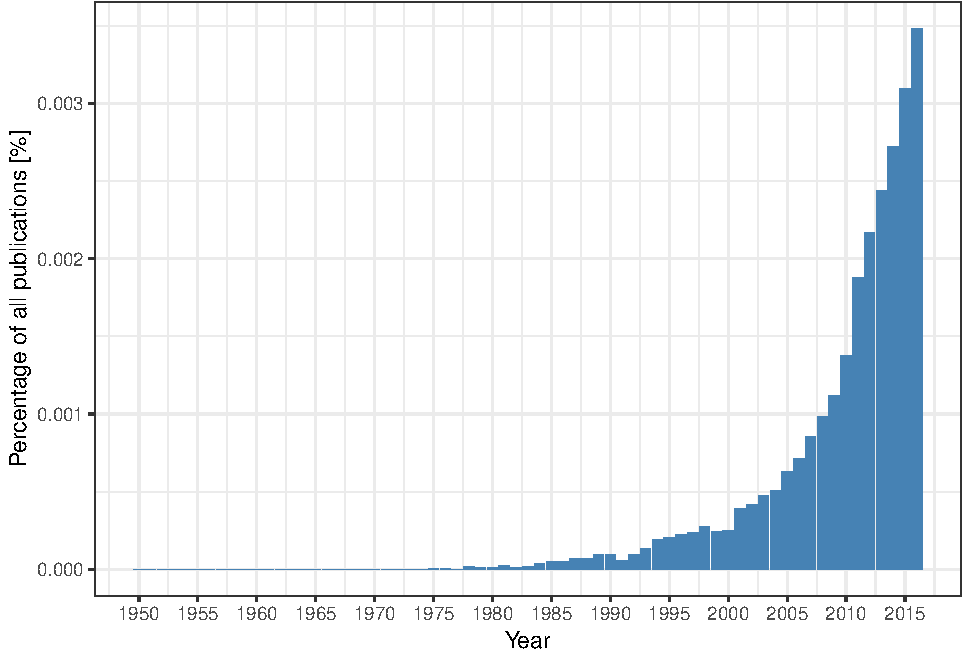
\includegraphics[width=0.7\linewidth]{UCzPhDThesis_files/figure-latex/pubmedTME-1} 

}

\caption{Percentage of publications containg phrase
``tumor immunotherapy'' is growing, numbers retreived on 17.01.2018 from
\href{http://dan.corlan.net/medline-trend.html}{Medline Trends}
\citep{Corlan2004}}\label{fig:pubmedTME}
\end{figure}






\hypertarget{tumor-micro-environment-fiend-or-foe}{%
\subsection{Tumor micro environment: fiend or
foe?}\label{tumor-micro-environment-fiend-or-foe}}

\hypertarget{what-is-tumor-microenvironment-tme}{%
\subsubsection{What is Tumor Microenvironment
(TME)}\label{what-is-tumor-microenvironment-tme}}

Tumor Microenvironment is a complex tissue that surrounds tumor cells.
It is composed of blood and lymphatics vessels, epithelial cells,
mesenchymal stem cells, fibroblast, adipocytes and a wide variety of
immune cells. Their proportion and specific roles vary significantly
with tumor type and stage. Communication between the environmental cells
and the tumor is critical for tumor development and its impact on
patient's response to treatment.

\hypertarget{tme-as-tumor-allay}{%
\subsubsection{TME as tumor allay}\label{tme-as-tumor-allay}}

In 1863 Rudolf Virchow observed a link between chronic inflammation and
tumorigenesis. Accoriding to Virchov theory genetic damage would be the
``match that lights the fire'' of cancer, and the inflammation or
cytokines produced by immune cells should be the ``fuel that feeds the
flames'' \citep{Balkwill2001}. Therefore lymphocyte infiltration was
confirmed by subsequent studies as a hallmark o cancer. The question one
may ask is why our immune system does not defend the organism from tumor
cells as it does in a range of bacterial and viral infections? It is
mainly because of the ability of tumor cells to inhibit immune response
through activation of negative regulatory pathways (so called immune
checkpoints).

Many examples can be cited on how TME facilitates tumor development
(Fig. \ref{fig:met-dis}). For instance, in the early stages of
tumorigenesis some macrophage phenotypes support tumor growth and
mobility through TGF-beta signaling. Also, it was shown that NK cells
and myeloid-derived suppressor cells (MDSCs) have an ability to suppress
immune defence i.e.~immunosurveillance by dendritic cells (DCs), T cell
activation and macrophage polarisation and they promote tumor
vascularisation as well. \citep{Talmadge2013, Gabrilovich2012} They
create so-called niches that facilitates tumor colonization. Tregs and
myeloid-derived suppressor cells can negatively impact natural immune
defence and by these means allow growth and invasion of tumor cells
\citep{Taube2017a}. Another cell type, a part of ECM, fibroblast, or
more precisely Cancer Associated Fibroblasts (CAFs) have proven
pro-tumor functions in breast cancer where they enhance metastasis
\citep{Dumont2013}. The blood and lymphatic vessels maintain tumor
growth providing necessary nutritive compound to malignant cells.

\begin{figure}

{\centering \includegraphics[width=1\linewidth]{figures-ext/massive-dissemination} 

}

\caption{The microenvironment supports metastatic
dissemination and colonization at secondary sites. Different tumor sites
can communicate through exosomes realized by tumor cells and also immune
and stromal cells such as NK cells, CAFs and DCs. Reprinted by
permission from Springer Nature \citep{Quail2013} © 2013 Nature America,
Inc.~All rights reserved.}\label{fig:met-dis}
\end{figure}








According to \citep{Hanahan2012} immune and stroma cells participate in
almost all of Cancer Hallmarks \citep{Hanahan2000, Hanahan2012} : Most
of the hallmarks of cancer are enabled and sustained to varying degrees
through contributions from repertoires of stromal cell types and
distinctive subcell types.

\hypertarget{two-faced-nature-of-immune-cells}{%
\subsubsection{Two-faced nature of immune
cells}\label{two-faced-nature-of-immune-cells}}

In the 1960s, the immune surveillance theory hypothesised ``the ability
to identify and destroy nascent tumors as a central asset of the immune
system'' \citep{Sebeok1976, Burnet1970}, but it was hihly criticised in
consequence of no increase in tumor incidence in athymic nude mice
{[}\citet{Stutman1974}; Rygaard1976{]}. Later it was shown, that this
mice model was not adequate \citep{Cavallo2011}. Over the years, it was
shown that the immune surveillance theory was not wrong, but was not
completely right neither.

Recent studies unveil ambivalent nature of immune cells of TME. While
some as cytotoxic T cells, B cells and macrophages can manage to
eliminate tumor cells. Treg cells role is to regulate expansion and
activation of T and B cells. Depending on cancer type, they can be
either pro- or anit- tumor. For example as it has been shown for Tregs,
they can be also associated with improved survival (i.e.~in colorectal
cancer \citep{Frey2010}. For innate immunity, there are widely accepted
M1 (ani-tumor) and M2 (pro-tumor) extreme macrophages phenotypes in TME
\citep{Qian2010}. Most of the statements seem to be context dependent
and not valid universally across all cancer types. We already mentioned
Macrophages phenotypic plasticity as well as different behaviour of EMC
depending on tumor stage.

From more general point of view, it has been observed that
immunodeficiency can correlate with high cancer incidence. Results of
analysis based on observations of 25,914 female immunosuppressed organ
transplant recipients, the tumor incidence was higher than predicted for
multiple cancers. However, the number of breast cancer cases decreased
which can be really disturbing if we need to decide on the role of
immune defence in tumor progression \citep{Stewart1995}. This trend was
confirmed through a study on individuals with AIDS and other studies.
This indicates that immune microenvironment can be cancer stimulating or
inhibiting depending on the type of cancer.

\hypertarget{cancer-immune-phenotypes}{%
\subsection{Cancer immune phenotypes}\label{cancer-immune-phenotypes}}

Since 20. century physicians decided on common nomenclature that
classify tumors into distinct groups that are relatively homogenous or
that share common characteristic important for treatment and prognosis.
Tumor typing should help to better asses predicting prognosis, to adapt
a therapy to the clinical situation, to enable therapeutic studies which
are essential in proving any therapeutic progress.

Most of the classifications are based on clinical data. Most common
factors taken into account are: the degree of local invasion, the degree
of remote invasion, histological types of cancer with specific grading
for each type of cancer, possibly various tumour markers, general status
of the patient.

With a progress of molecular biology also gene markers or proteomic
abnormalities can be part of classification panel.

Since the increase of importance of the immunotherapies, researches
proposed several ways to classify tumors based on their
microenvironment. Given different parameters describing TME, cancers can
be sorted into groups that show similar characteristics. We will discuss
most common frameworks that allow to phenotype cancers based on the TME.

The localisation of the immune cells can be an indicator of the state
and response to the therapy \citep{Bindea2013}.

The most standard approach is to convey an analysis of histopathological
cuts to asses the number of infiltrating lymphocytes (TILs). Two typical
patterns are usually identified: ``hot'' - immune inflamed and ``cold''
- no active immune response \citep{Berghoff2018}.

\citet{Chen2017} describes classification into inflamed and non-inflamed
tumors, where non-inlamed phenotypes: can be further split into the
immune-desert phenotype and the immune--excluded phenotype (Fig.
\ref{fig:immune-phenotypes}). The inflamed phenotype is characterised by
rich presence of immune cells : T cells, myeloid cells, monocytes in
tumor margin. Along with the immune cels, due to their communication, a
high expression of cytokines is characteristic for this phenotype.
According to Chen2017, this is a mark of anti-tumor response that was
arrested by tumor. The inflamed phenotype has shown to be most
responsive to immunotherapies. In the immune-excluded phenotype, the
immune cells are present as well but located in the stroma
\citep{Herbst2014}, sometimes penetrating inside tumor. However, when
exposed to check point immuotherapy, T cells does not gain the ability
to infiltrate the tumor, therefore the treatment is inefficient. The
immune-desert main features is little or no presence of immune cells,
especially T cells. Surprisingly, this tumors have been to proven to
rarely respond to the checkpoint therapy \citep{Herbst2014}. In
non-inflamed tumours cytokines associated with immune suppression or
tolerance are expressed.

\begin{figure}

{\centering 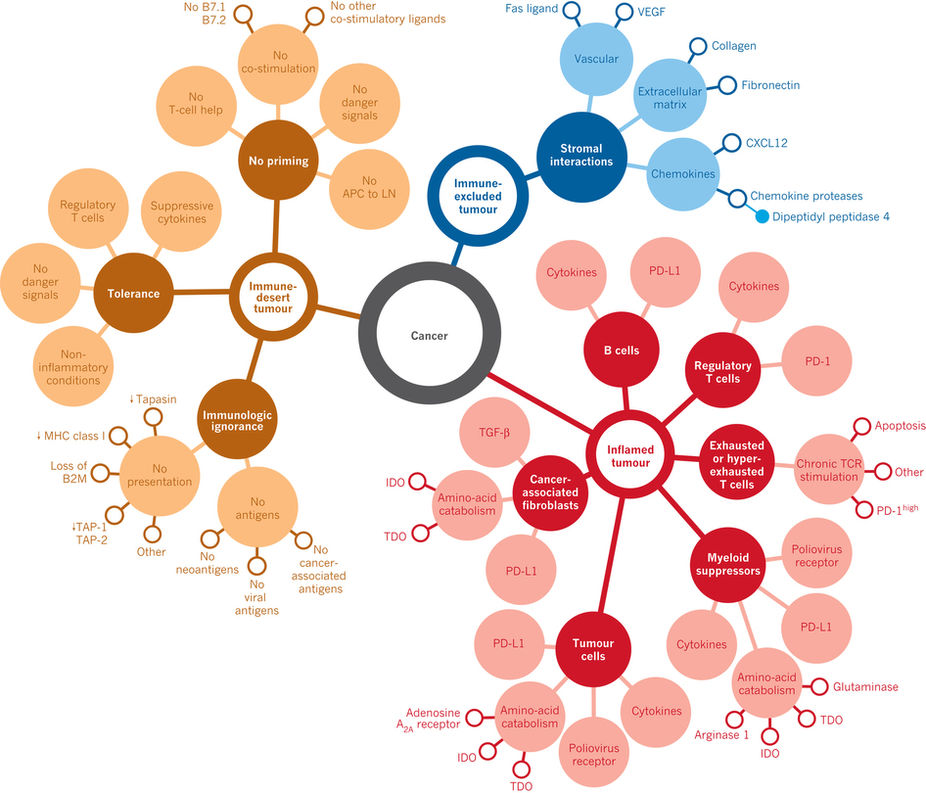
\includegraphics[width=1\linewidth]{figures-ext/immune-phenotypes} 

}

\caption{Cancer-immune phenotypes: the
immune-desert phenotype (brown), the immune--excluded phenotype (blue)
and the inflamed phenotype (red). The immune--desert phenotype is
characterised by paucity of immune cells and cytokines. In the
immune-excluded phenotypes the T cells are often present but trapped in
stroma, enabled to migrate to the tumor site. The immune-inflamed
phenotype is rich in immune cells and the most responsive to the immune
check point therapies. Reprinted by permission from Springer Nature
\citep{Chen2017} © 2017 Macmillian Publishers Limited, part of Springler
Nature. All rights reserved.}\label{fig:immune-phenotypes}
\end{figure}












The immunogenicity of the tumors can be explained by tumor-intrinsic
factors and tumor-extrinsic factors \citep{Gajewski2006}.
Tumor-intrinsic factors are, the neoantigen load and frequency, the
mutational load, the expression of immunoinhibitors and
immunostimulators (e.i. PD-L1), and alteration of HLA class I molecules.
Tumor-extrinsic factors include chemokines regulating T cell
trafficking, infiltration of effector TILs and immunosuppressive TILs,
and soluble immunomodulatory factors (cytokines).

A plethora of different computational methods have been developed in
order to further characterise tumor samples using different factors. We
mention here mainstream methods that cover different approaches of
scoring the TME-cancer phenotype.

\hypertarget{immunoscore}{%
\subsubsection{Immunoscore}\label{immunoscore}}

Image-based tumors classification

\url{http://www.haliodx.com/clinical-research-services/immunoscorer/}

\citet{Galon2012}

\hypertarget{immunophenoscore}{%
\subsubsection{Immunophenoscore}\label{immunophenoscore}}

Different approaches are based on gene expression patterns. Most
commonly, machine learning supervised algorithms are trained to match
known phenotype (established with microscopy or with clinical features)
to genetic patterns or an unsupervised clustering is used to discover
new classification.

An example of well-formulated classification framework is
Immunophenoscore \citep{Charoentong}, based on publication of
\citet{Angelova2015}, where methylome, transcriptome and mutation of
TCGA CRC dataset (n = 598) was used to describe \emph{immunophenotypes}.
Later on, it was reduced to gene expression indicator and summarised in
a form of a score. In This scoring scheme is based on the data of 20
solid tumors, using expression of marker genes selected by a Machine
Learning algorithm (random forest) for best prediction in each cancer.
These indicators can be grouped into four categories:

\begin{itemize}
\tightlist
\item
  MHC molecules (MHC)
\item
  Immunomodulators (CP)
\item
  Effector cells (EC)
\item
  Suppressor cells (SC)
\end{itemize}

The immunophenscore (IPS) is calculated on a 0-10 scale based on the
expression of genes in each category. Stimulatory factors (cell types)
impact the score positively and inhibitory factors (cell types)
negatively. Z-scores ≥ 3 were designated as IPS10 and z-scores ≤ 0 are
designated as IPS0. A similar conceptual framework called \emph{cancer
immunogram} was proposed by \citet{Blank2016} included seven parameters:
tumor foreignness (Mutational load), general immune status (Lymphocyte
count), immune cell infiltration (Intratumoral T cells), absence of
checkpoints (PD-L1), absence of soluble inhibitors (IL--6, CRP), absence
of inhibitory tumor metabolism (LDH, glucose utilisation), tumor
sensitivity to immune effectors (MHC expression, IFN-γ sensitivity).
Nonetheless, the details of \emph{cancer immunogram} use in practice
remain unclear and result could be sensitive to patients' and data
heterogeneity as no standardisation was proposed.

\citet{Charoentong} claim that the immunophenoscore can predict response
to CTLA-4 and anti-PD-1.

\hypertarget{immune-maps}{%
\subsubsection{Immune maps}\label{immune-maps}}

Description on how immune portraits (NAVIcell) can be used to
characterise tumor immune environment.

Despite those facts, the gene expression based classifications are not
yet used in clinics. The measured multi-panel mRNA expression, that can
be included into category of In Vitro Diagnostic Multivariate Index
Assay (IVDMIA) \citep{Gyorffy2015, Ross2008}, may be a future of
TME-based cancer classification, diagnosis and treatment recommendation
\citep{Gnjatic2017}. For this best tools need to be used to properly
evaluate the state of TME and tumor-stroma-immune cells communication.

\hypertarget{immune-signatures}{%
\subsection{Immune signatures - biological
perspective}\label{immune-signatures}}

\begin{itemize}
\tightlist
\item
  definition of signature: marker genes, list of genes, weighted list,
  metagenes
\item
  the general immune signature of signature of immune infiltration and
  stroma vs immune signature of a specific cell type of functional
  subpopulation
\item
  purpose of signatures
\item
  availability of immune signatures
\item
  the problem of not consistency of immune signatures
\item
  origin of signatures
\end{itemize}

\begin{quote}
``the gene expression profiles of tumour-associated immune cells differ
considerably from those of blood derived immune cells'''
\citep{Schelker2017}
\end{quote}

Immune signatures will be also discussed as a part of deconvolution
pipeline in the \protect\hyperlink{methods}{Chapter 2}.

\hypertarget{immunotherapies}{%
\section{Immunotherapies}\label{immunotherapies}}

This section outlines progress in cancer therapies with a focus on
immune therapies. It will link the ongoing research on TME with
therapeutical potential.

\hypertarget{cancer_Therapies}{%
\subsection{Cancer therapies}\label{cancer_Therapies}}

Cancer is a complex disease. Up to date, no uniform and fully effective
treatment was proposed and usually different strategies are tested to
kill tumor cells. \textbf{Surgery} is one of the oldest methods. The
cancer is removed from the patient body. There are different ways, more
or less invasive, that it can be performed. it is usually applied for
solid tumor contained in a small area. \textbf{Radiation Therapy} uses
high doses of radiation to eliminate tumor cells and shrink tumor mass.
It can be applied externally or internally. \textbf{Chemotherapy} uses a
drug (or a combination of drugs) that kill cancer cells, usually
altering cell proliferation and growth. The drawback of radiotherapy and
chemotherapy are strong side effects. \textbf{Hormone therapy } modulate
hormone levels in the body in order to inhibit tumor growth in breast
and prostate cancers. In leukemia and lymphoma, can be applied
\textbf{stem cell transplants} that restore blood-forming stem cells
destroyed by the very high doses of chemotherapy or radiation therapy
that are used to treat certain cancers.

Alternatively, \textbf{targeted therapies} represent more focused
strategy that aims to be more effective and cause less side effects than
systematic therapies. Two main types of targeted therapies are
small-molecule drugs and monoclonal antibodies. Targeted therapies
usually aim to stimulate/inhibit a selected molecular function. A
special types of targeted therapies are \textbf{Immunotherapies}.
Through adtivation/inhibition of immune regulatory pathways, it
stimulates immune system to destroy malignant cells. A continuation of
targeted therapies is \textbf{precision medecine approach}. It is based
on genetic information to specify patient's profile and find adapted
treatment. A number of innovative treatments targeting a specific change
in tumor ecosystem are being tested presently in precision medicine
clinical trials \citep{NCI2018}.

\hypertarget{recent-progress-in-immuno-therapies}{%
\subsection{Recent progress in
immuno-therapies}\label{recent-progress-in-immuno-therapies}}

The immunotherapies, in contrast with other types of cancers therapies
discussed in \protect\hyperlink{cancer_Therapies}{the previous chapter},
aim to trigger or restart the immune system to defend the organism and
attack the malignant cells. All this, however without provoking
persisting inflammation state \citep{Predina2013}

The idea of stimulating immune system to fight malignant cell was not
born recently. Since a long time a possibility of development of an
anti-cancer vaccine has been investigated. Unfortunately, this idea
faced two important limitations 1) lack of knowledge of antigens that
should be used in vaccine to successfully stimulate cytotoxic T cells 2)
the ability of cancer to block the immune response also called
\emph{immunostat}. Despite those impediments works on anti-tumor
vaccines do not \citep{Palucka2013}.

Another idea involving using immune system as a weapon to fight cancer,
would be the use of genetically modified patient's T-cells, carrying
\emph{CARs} (chimeric antigen receptors) \citep{Jackson2016}. After a
long period of small unsuccessful trials, recently in 2017, two CAR
T-cell therapies were accepted, one to ``treat adults with certain type
of large B-cell lymphoma'' \citep{FDACARTadult}, other to treat
``children with acute lymphoblastic leukemia (ALL)'' \citep{FDACARTALL}
, which are, at the same time, the first two gene therapies accepted by
FDA.

However, the two most promising immuno-related strategies are based on
blocking so called immune check point inhibitors: cytotoxic T-lymphocyte
protein 4 (CTLA4) and programmed cell death protein 1 (PD-1). The
anti-CLTA4 antibodies blocks repressive action of CLTA4 on T-cells and
they become therefore activated. It was shown efficient in melanoma
patients and accepted by FDA in 2015 as adjuvant therapy for stage III
metastatic melanoma patients \citep{FDACTLA4}. PD-1 is a cell surface
receptor of T cells, that binds to PD-L1/PD-L2. After binding, an
immunosuppressive pathway is activated and T cells activity is dampened.
An action of an anti-PD-L1 antibody is to prevent this immune exhaustion
\citep{Chen2017}. A stepping stone for anti-PD-L1 therapies was approval
of Tecentriq (atezolizumab) for Bladder cancer \citep{FDAPDL1Bladder}
and anit-PD1 Keytruda (pembrolizumab) initially accepted for NSCLC and
further extended to head and neck cancer, Hodgkin's lymphoma, gastric
cancer and microsatellite instability-high cancer \citep{FDAPDL1NSCLC}.
Since other anti-PD-L1 or anti-PD1 antibodies were accepted or entered
advanced stages of clinical trials \citep{Wolchok2015}. A short history
of immunotherapy FDA-accepted treatments can be found in Fig.
\ref{fig:timeline-immunotherapies}

\begin{figure}

{\centering 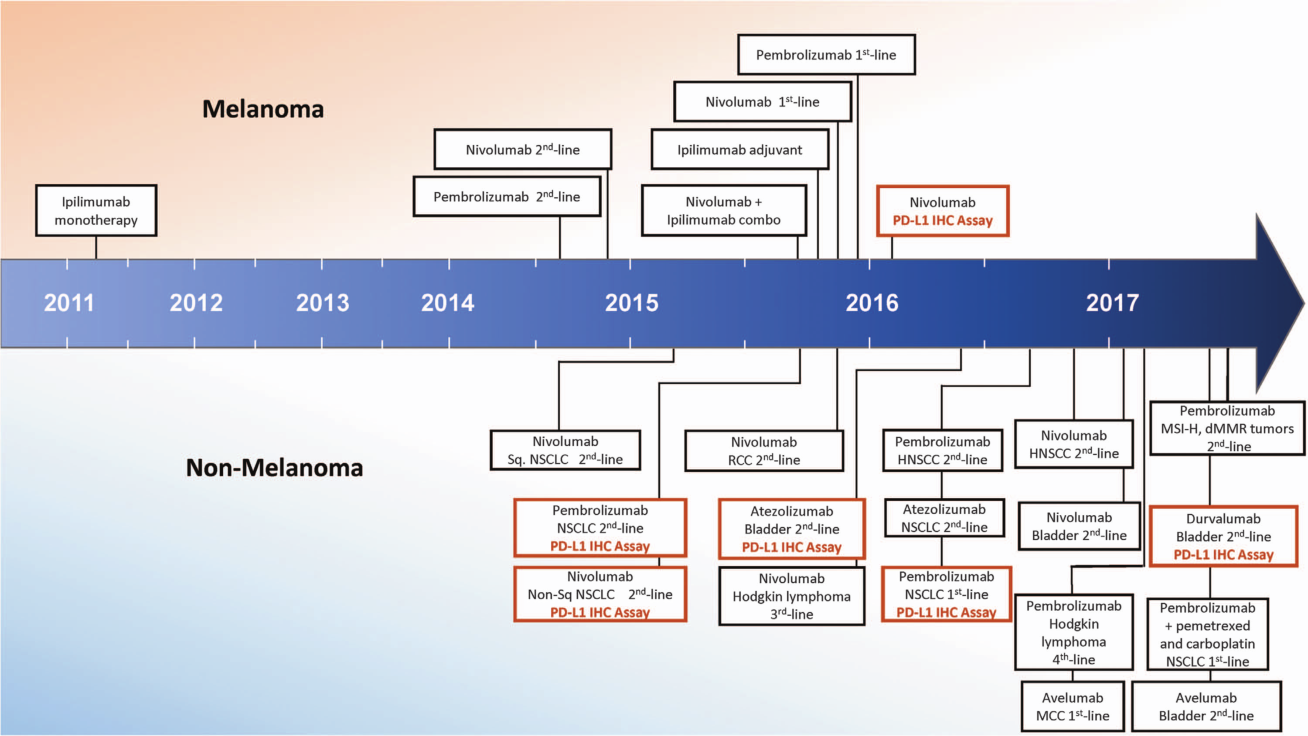
\includegraphics[width=1\linewidth]{figures-ext/02-timeline-immunotherapies} 

}

\caption{This timeline describes short
history of FDA approval of checkpoint blocking immunotherapies up to
2017. Reprinted by permission from Springer Nature \citep{Taube2017a}
Macmillan Publishers Limited, part of Springer Nature. All Rights
Reserved.}\label{fig:timeline-immunotherapies}
\end{figure}







The main drawback of immunotherapies is a heterogeneity of response
rate, which can vary i.e.~from 10--40\% in case of PD-L1blocking
\citep{Zou2016}, suggesting that some patient can have more chances than
others to respond to an immune therapy. So far, it has been shown that
anti PD-L1 therapies works more effectively in T cell infiltrated tumors
with exclusion of Tregs because of lack of difference in expression of
FOXP3 in responding and non-responding group of patients
\citep{Herbst2014}. Also some light has been shade by \citet{Rizvi2015}
who connected mutational rate of cancer cells to the chances of response
to an immunotherapy.

Despite those fundings, the precise qualifications of patients that
should be sensitive to an immunotherapy are not defined
\citep{Pitt2016}. As most patients do not answer to immunotherapies, it
stimulates researches to look for better biomarkers and patient
stratifications, and pharmaceutical industries to discover new immune
checkpoints based therapies.

\hypertarget{quantifying-immune-infiltration-data}{%
\section{Quantifying immune infiltration
(data)}\label{quantifying-immune-infiltration-data}}

Nowadays, more and more biological data is produced. However, this
proliferation of accessible resources is not proportional to generated
insights and wisdom. In this thesis, we wok mostly generate
\emph{Knowledge} and \emph{Insights} and we hope to generate some
\emph{Wisdom} (Fig. \ref{fig:information-power}). However, in this part,
we will introduce the foundation of our analysis: different data types
that will be further discussed in chapters that follow.

\begin{figure}

{\centering 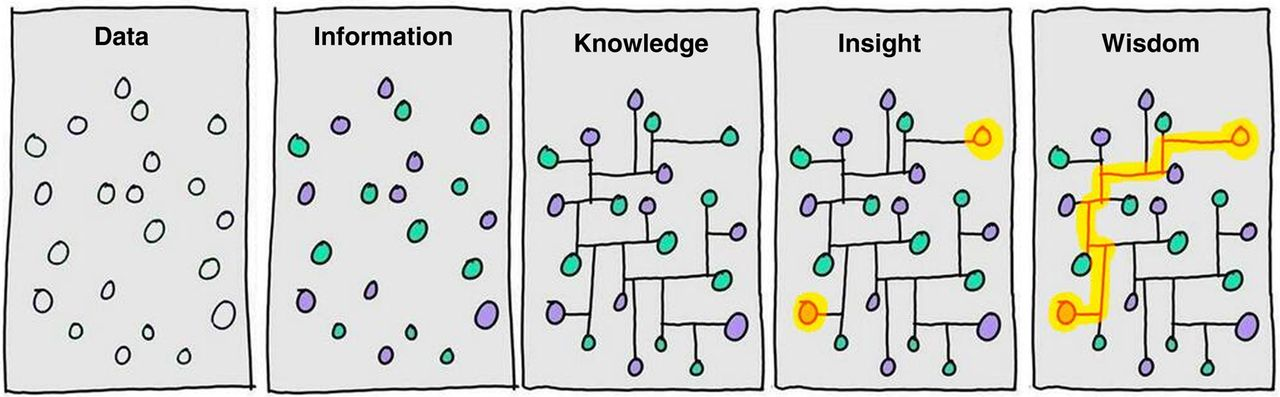
\includegraphics[width=0.8\linewidth]{figures-ext/01-Information_power} 

}

\caption{\textbf{From \emph{Data} to
\emph{Wisdom}}. Illustration of different steps that it takes to go from
\emph{Data} to generating \emph{Wisdom}. It highlights that generating
data is not equal to understanding it and additional efforts are needed
to generate value. Image authored by Clifford Stoll and Gary Schubert
published by Portland Press Limited on behalf of the Biochemical Society
and the Royal Society of Biology and distributed under the
\href{https://creativecommons.org/licenses/by/4.0/}{Creative Commons
Attribution License 4.0 (CC-BY)} in \citep{Ponting2017}.}\label{fig:information-power}
\end{figure}











We will introduce most relevant data types that are used to study immune
infiltration of tumors.

\hypertarget{facs}{%
\subsection{Cell sorting}\label{facs}}

\hypertarget{flow-cytometry}{%
\subsubsection{Flow cytometry}\label{flow-cytometry}}

Flow cytometry is a laser-based technology. It uses marker genes: cell
surface proteins to sort cells in different compartments. Nowadays, it
permits quantification of the abundance of up to 17 cell surface
proteins using fluorescently labelled antibodies \citep{Papalexi2017}.

\hypertarget{mass-cytometry}{%
\subsubsection{Mass cytometry}\label{mass-cytometry}}

Mass cytometry (also known as CyTOF allows for the quantification of
cellular protein levels by using isotopes. It allows to quantify up to
40 proteins per cell \citep{Papalexi2017}.

\hypertarget{staining}{%
\subsection{Microscope Staining}\label{staining}}

Using microscope technics, histopathological cuts are analysed. The
number of cells per a unit of area (i.e.~mm\(^2\)) is defined either
manually by human or though diverse image analysis algorithms. Current
pathology practice utilises chromogenic immunohistochemistry (IHC)
\citep{RamosVara2010}. Multiplexed approaches allow to identify multiple
markers in the same histopathology cut. Modern techniques as imaging
mass cytometry using FFPE tissue samples uses fluorescence and mass
cytometry to identify and quantify marker proteins \citep{Giesen2014}.

The main advantage of aforementioned technics the number of cells that
can be analysed and the information about spatial distribution of the
different cell types. The limiting factor, as for
\protect\hyperlink{facs}{cell sorting methods}, is the number of markers
(\textasciitilde{}10-100) and consequently number of cell types that can
be identified \citep{Schelker2017}.

The \protect\hyperlink{facs}{cell sorting methods} and
\protect\hyperlink{staining}{microscope staining} are usually considered
as a gold standard for multidimensional data techniques. The reason why
they are not applied at large scale is the cost but also quite laborious
and time consuming sample preparation demanding a fresh sample. In
contrast, the \protect\hyperlink{omics}{-omics methods} propose more
scalable way to measure tumor micro environment.

\hypertarget{omics}{%
\subsection{omics}\label{omics}}

\begin{itemize}
\tightlist
\item
  Some kind of sequencing explanation needed for non-biologists
\end{itemize}

\hypertarget{transcriptome}{%
\subsubsection{Transcriptome}\label{transcriptome}}

Transcriptomics is measures the number of counts of mRNA molecules using
high-throughput techniques. mRNA is the part of genetic information that
should be translated to proteins. It reflects the activity of cell
ongoing processes. In contrast to DNA, mRNA is highly variant
\citep{Velculescu1997}. In addition, many genetic and epigenetic events
can be either directly observed or indirectly inferred from
transcriptomic data. Transcriptome can be measure with microarrays or
RNA-seq NGS technology.

Bulk transcriptome data can are quite accessible. They can be obtained
from either flash-frozen or formalin-fixed, paraffin-embedded (FFPE)
tissue samples, including both surgically resected material and core
needle biopsies \citep{Schelker2017}.

The main flaw of transcriptomic data is that the reproducibility between
different platforms is limited. As a result, direct comparison between
two datasets produced by different platforms is not advised.

Different strategies can be adapted to analyse bulk transcriptome.

\citet{Cieslik2017} describes five groups of most popular approaches
that can be applied to study transcriptome (Fig.
\ref{fig:transcriptome-methods}). Despite a diversity of bioinformatic
and statistical tools, the most popular differential approaches, mainly
differential gene expression (DGE) based on difference between two
experimental conditions.

\begin{figure}

{\centering 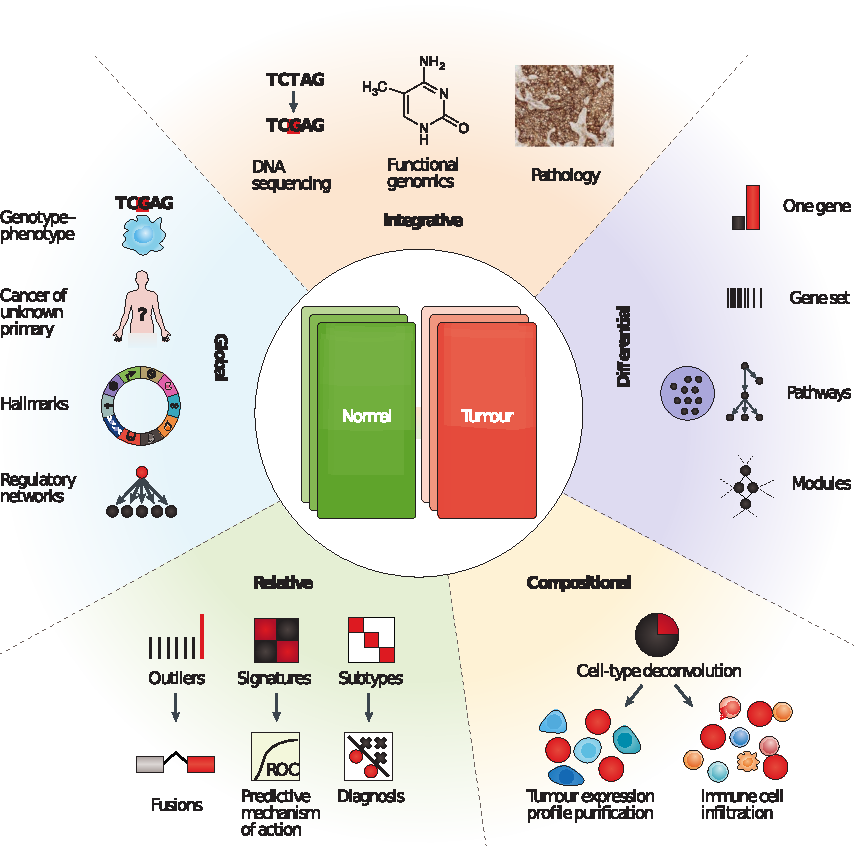
\includegraphics[width=1\linewidth]{figures-ext/transcriptome-methods} 

}

\caption{Five categories of RNA-seq data
analysis. Differential analyses: comparing two (or more) conditions,
Relative analyses: comparing to an internal refernce (average, base
level), Compositional analyses: inferring cell types or groups of cell
types (i.e.~tumor purity), Global analyses: pan-tissue and pan-cancer
analyses and Integrative analyses: compiling heterogneious data types.
Reprinted by permission from Springer Nature \citep{Cieslik2017} © 2018
Macmillian Publishers Limited, part of Springler Nature. All rights
reserved.}\label{fig:transcriptome-methods}
\end{figure}











RNA-seq data was proven to be a useful indicator for clinical
applications \citep{Mody2015, Oberg2016, Robinson2017}. Its utility for
immune profiling was demonstrated in may studies through a use of
transcriptomic signatures to predict immunotherapy response or survival
\citep{Chen2016}.

In this work transcriptome data are analyzed propose an alternative
method to describe immune infiltration.

\hypertarget{epigenome}{%
\subsubsection{Epigenome}\label{epigenome}}

An epigenome can be defined as a record of the chemical changes to the
DNA and histone proteins of an organism. Changes to the epigenome can
provoke changes to the structure of chromatin and changes to the
function of the genome \citep{Bernstein2007}. Epigenome data usually
contains information about methylation CpG island changes. In cancer,
global genomic hypomethylation, CpG island promoter hypermethylation of
tumor suppressor genes, an altered histone code for critical genes, a
global loss of monoacetylated and trimethylated histone H4 were
observed. Mathylome profiles can be also use as molecular signature
{[}NMF and other ref{]}

\hypertarget{single-cell-rna-seq}{%
\subsubsection{Single cell RNA-seq}\label{single-cell-rna-seq}}

Described above methods of process DNA from hundreds of thousands of
cells simultaneously and report averaged gene expression of all cells.
In contrast, scRNA-seq technology allows getting results for each cell
individually. This is tremendous step forward enhancement of our
understanding of cell heterogeneity and opens new avenues of research
questions.

Continuous discovery of new immune subtypes has proven that cell surface
markers that are used for phenotyping by techniques like
\protect\hyperlink{facs}{FACS} and
\protect\hyperlink{staining}{immunohistochelistry} cannot capture the
full complexity. ScRNA-seq methods allow to cluster known cell types in
subpopulations based on their genetic features \citep{Papalexi2017}.
ScRNA-seq is also able to capture particularly rare cell types as it
requires much less of RNA material (1 ng isolated from 100-1000 cells)
compared to `bulk' RNA-seq ( \textasciitilde{} 1 μg of total mRNA
transcripts ). It also allow to study cells at high resolution where the
phenotypes can re-defined in much more refined scale than previously
\citep{Papalexi2017}

This new data type also brings into the field new challenges related to
data processing due to the volume, distribution, noise, and biases.
Experts highlight as the most ``batch effect'', ``noise'' and ``dropout
effect'' \citep{Perkel2017}. So far, there are no official standards
that can be applied which makes data comparison and post-processing even
more challenging. Up to date, there are around 70 reported tools and
resources for single cell data processing \citep{Davis2016} .

A limited number of single-cell datasets of tumors are made publicly
available (@ TABLE ?).

One can ask why then developing computational deconvolution of
transcriptome if we can learn relevant information from single-cell
data. Today's reality is that single cell data does not provide a
straightforward answer to the estimation of cell proportions. The
coverage is not full and sequenced single cells are not fully
representative of the true population. For instance, neutrophiles are
not found in scRNA-seq data because of they are ``difficult to isolate,
highly labile \emph{ex vivo} and therefore difficult to preserve with
current single-cell methods'' \citep{Schelker2017}. In addition, a
number of patients included in published studies of range \textless{}100
cannot be compared to thousand people cohorts sequenced with bulk
transcriptome methods. This is mostly because single cell experiments
are challenging to perform, especially in clinical setting as fresh
samples are needed \citep{Schelker2017}. Today, single cell technology
brings very interesting ``zoom in'' perspective, but it would be
incautious to make fundings from a restricted group of individuals
universal to the whole population. Major brake to the use of single cell
technology more broadly might be as well the price that is neatly 10x
higher for single cell sample compared to bulk \citep{Cedar2018}.

\begin{longtable}[]{@{}cc@{}}
\toprule
Technology & Price\tabularnewline
\midrule
\endhead
scRNA-seq & 3000\$ / sample\tabularnewline
RNA-seq & 200 \$ / sample\tabularnewline
FACS & 0.05\$ / cell\tabularnewline
CyTOF & 35\$/cell\tabularnewline
\bottomrule
\end{longtable}

In this work, we are using single cell data in two ways. Firstly, in
\protect\hyperlink{results}{Comparative\ldots{} chapter} we compare
immune cell profiles defined by scRNA-seq, blood and blind deconvolution
(problem introduced in \protect\hyperlink{immune-signatures}{Immune
signatures section}). Secondly, in \protect\hyperlink{map}{Heterogeneity
of immune\ldots{}} we use single call data of Metastatic melanoma
generated by \citet{Tirosh2016} to demonstrate subpopulations of
Macrophages and NK cells.

\hypertarget{methods}{%
\chapter{Mathematical foundation of cell-type deconvolution of
biological data}\label{methods}}

In this chapter, we will discuss how mathematical models can be used to
extract information about specific cell-types from `bulk' data or how to
unmix mixed sources. It will introduce you to basic concepts of data
analysis as well as most popular advanced solutions adapted for
estimating presence and proportion of immune cells within cancer
biopsies.

\hypertarget{introduction-to-supervised-and-unsupervised-learning}{%
\section{Introduction to supervised and unsupervised
learning}\label{introduction-to-supervised-and-unsupervised-learning}}

\hypertarget{blind-source-sepration}{%
\section{Blind source sepration}\label{blind-source-sepration}}

(ICA, NMF etc)

\hypertarget{finding-optimal-number-of-components-and-over-decomposition-of-transcriptopmes}{%
\section{Finding optimal number of components and over-decomposition of
transcriptopmes}\label{finding-optimal-number-of-components-and-over-decomposition-of-transcriptopmes}}

(adapted from BMC article)
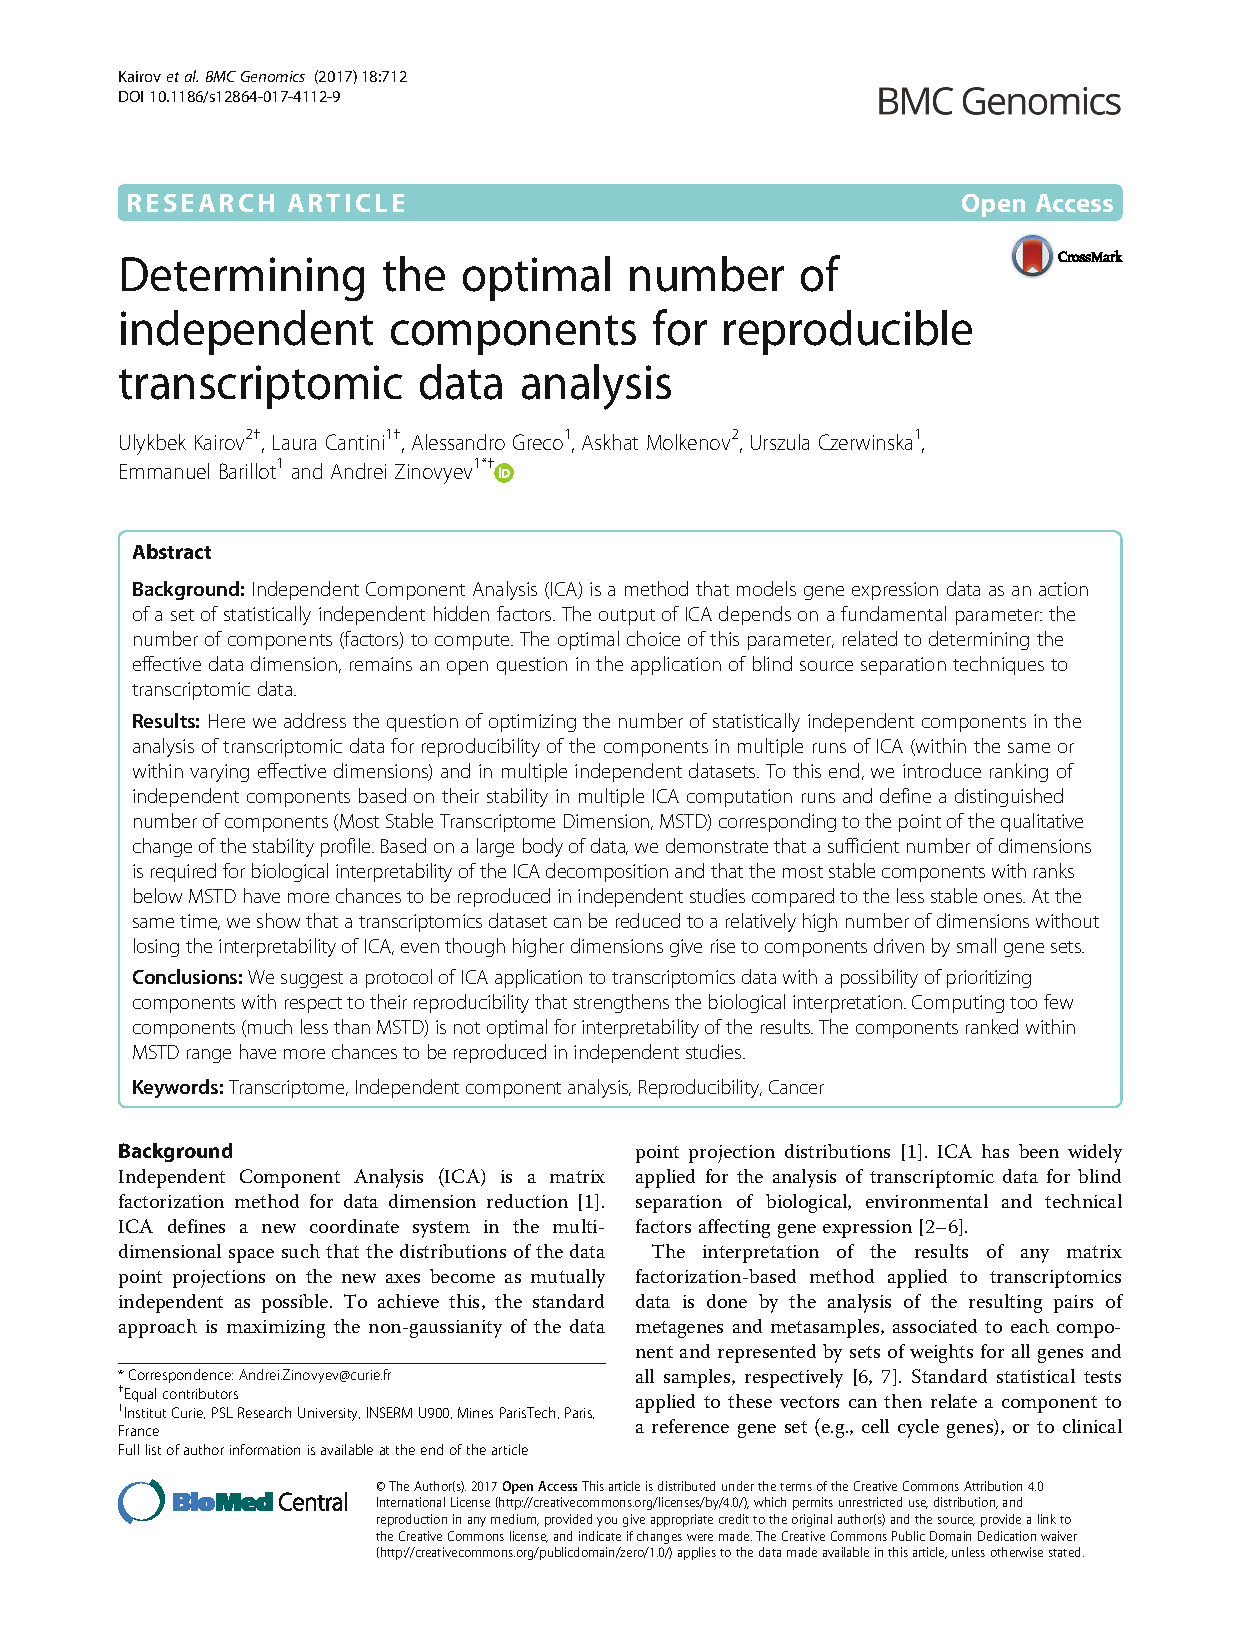
\includepdf[pages={1-}, scale=1]{pdf-ext/BMCMSTD.pdf}

\hypertarget{cell-type-deconvolution-models}{%
\section{Cell-type deconvolution
models}\label{cell-type-deconvolution-models}}

(families of approaches)

\hypertarget{basis-matrix}{%
\subsection{basis matrix}\label{basis-matrix}}

\hypertarget{regression-algorithm}{%
\subsection{regression algorithm}\label{regression-algorithm}}

\hypertarget{others}{%
\subsection{others}\label{others}}

\hypertarget{short-review-of-most-popular-cell-type-deconvolution-tools}{%
\section{Short review of most popular cell-type deconvolution
tools}\label{short-review-of-most-popular-cell-type-deconvolution-tools}}

tools will already be mentioned in the section above. However a comment
on other than mentionned aspects are needed

\hypertarget{study-of-sensitivity-of-known-methods}{%
\chapter{Study of sensitivity of known
methods}\label{study-of-sensitivity-of-known-methods}}

\hypertarget{reproducibility-of-nmf-versus-ica}{%
\section{Reproducibility of NMF versus
ICA}\label{reproducibility-of-nmf-versus-ica}}

\hypertarget{impact-of-modification-of-signatures-list-on-result-for-signature-based-deconvolution-methods}{%
\section{Impact of modification of signatures list on result for
signature-based deconvolution
methods}\label{impact-of-modification-of-signatures-list-on-result-for-signature-based-deconvolution-methods}}

\hypertarget{deconvolution-of-transcriptomes-and-methylomes}{%
\chapter{Deconvolution of transcriptomes and
methylomes}\label{deconvolution-of-transcriptomes-and-methylomes}}

We describe our methods in this chapter. The pre-eliminary pipeline and
simple results are described in the manuscript submitted to
Springer-Verlag's Lecture Notes in Computer Science
(\href{http://www.springer.com/gb/computer-science/lncs}{LNCS}) entitled
\textbf{Application of Independent Component Analysis to Tumor
Transcriptomes Reveals Specific And Reproducible Immune-related Signals}
that is placed at the end of this chapter. In the final thesis final
pipeline will be split into following structure

\hypertarget{from-blind-deconvolution-to-cell-type-quantification-general-overview}{%
\section{From blind deconvolution to cell-type quantification: general
overview}\label{from-blind-deconvolution-to-cell-type-quantification-general-overview}}

\hypertarget{the-ica-based-deconvolution-of-transcriptomes}{%
\subsection{The ICA-based deconvolution of
Transcriptomes}\label{the-ica-based-deconvolution-of-transcriptomes}}

\hypertarget{interpretation-of-independent-components}{%
\subsection{Interpretation of Independent
components}\label{interpretation-of-independent-components}}

\hypertarget{correlation-based-identification-of-confunding-factors}{%
\subsubsection{Correlation based identification of confunding
factors}\label{correlation-based-identification-of-confunding-factors}}

\hypertarget{identification-of-immune-cell-types-with-enrichment-test}{%
\subsubsection{Identification of immune cell types with enrichment
test}\label{identification-of-immune-cell-types-with-enrichment-test}}

\hypertarget{transforming-metagenes-into-signature-matrix}{%
\subsection{Transforming metagenes into signature
matrix}\label{transforming-metagenes-into-signature-matrix}}

\hypertarget{regression-based-estimation-of-cell-type-proportions}{%
\subsection{Regression-based estimation of cell-type
proportions}\label{regression-based-estimation-of-cell-type-proportions}}

\hypertarget{deconica-r-package-for-ica-based-deconvolution}{%
\section{\texorpdfstring{\emph{DeconICA} R package for ICA-based
deconvolution}{DeconICA R package for ICA-based deconvolution}}\label{deconica-r-package-for-ica-based-deconvolution}}

This part of the chapter will be adapted from package vignettes

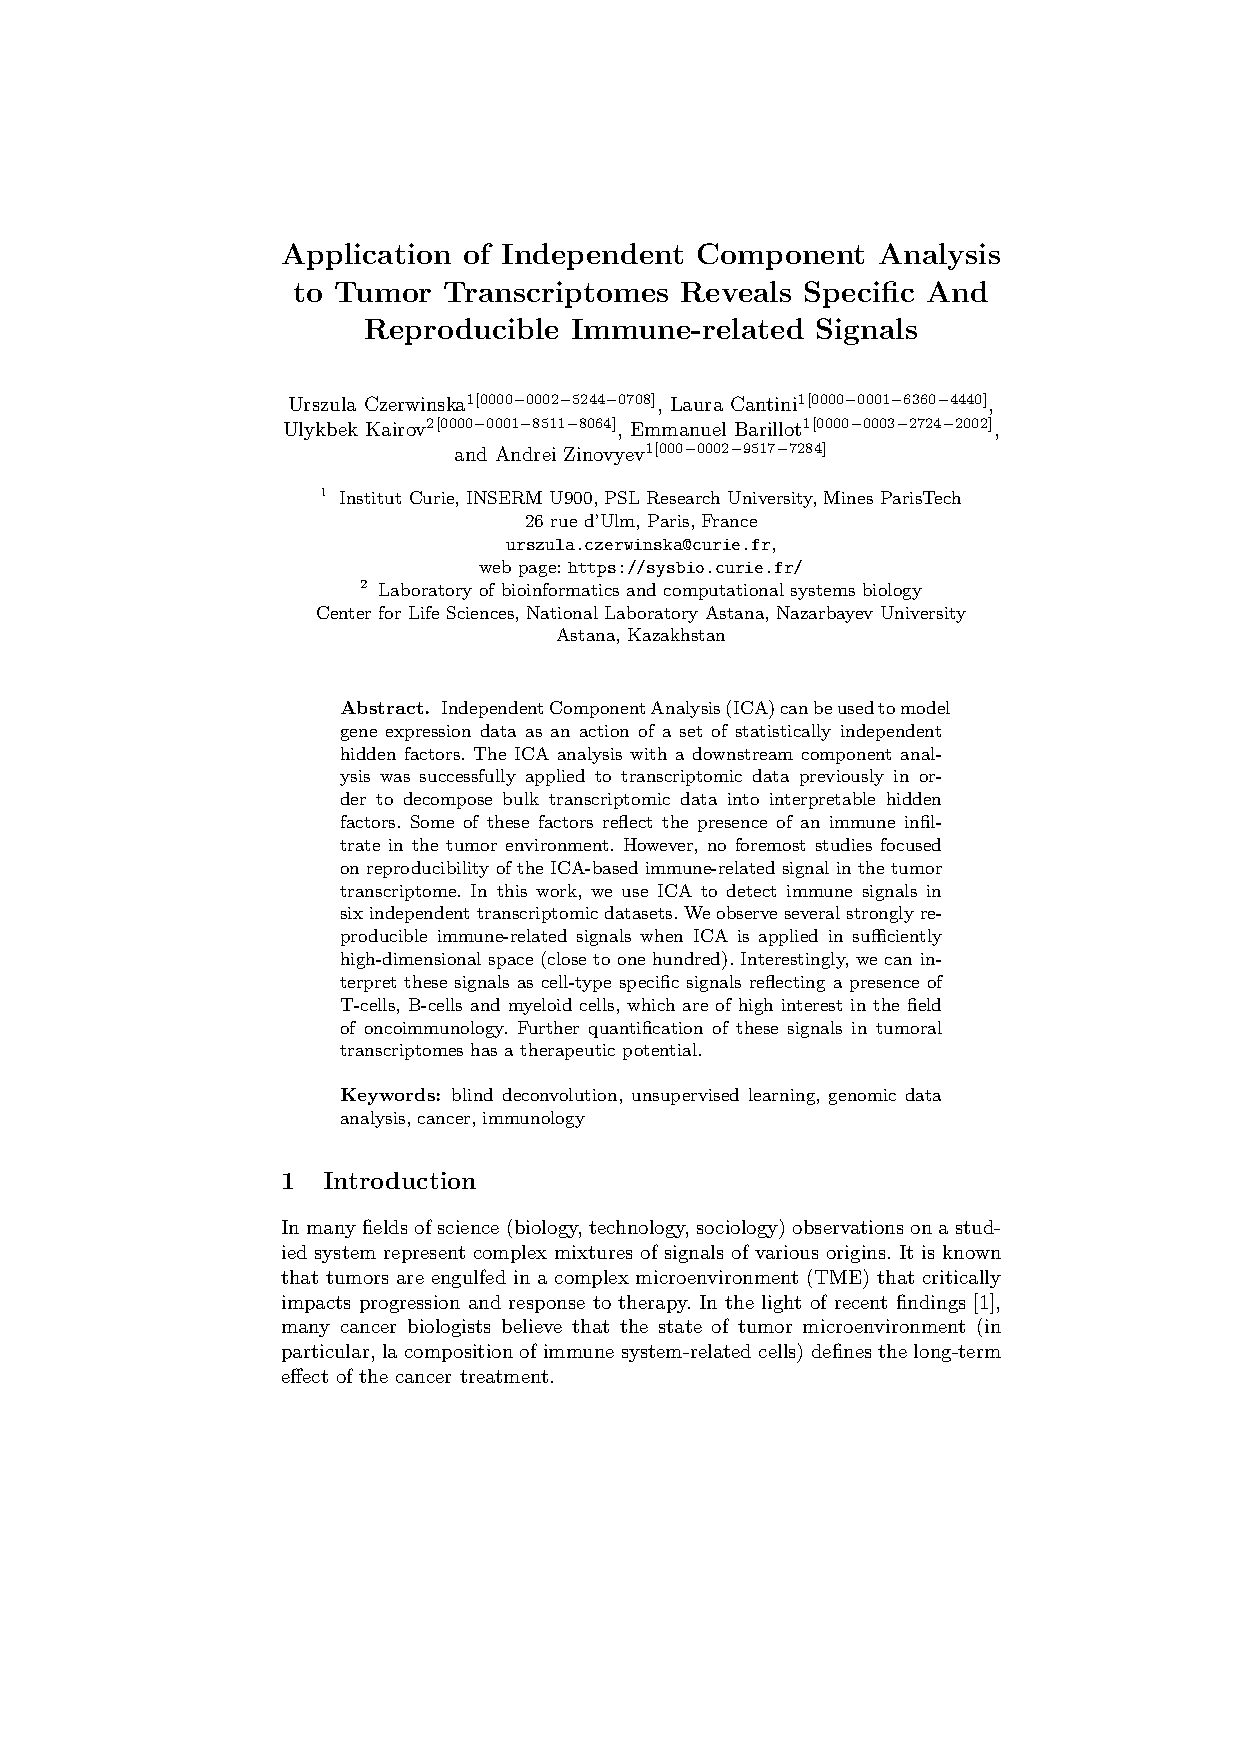
\includepdf[pages={1-}, scale=1]{pdf-ext/LVAICA.pdf}

\hypertarget{results}{%
\chapter{Comparative analysis of cancer immune
infiltration}\label{results}}

This chapter will include biological interpretation of Pan-cancer
analysis with DeconICA

\hypertarget{section}{%
\section{}\label{section}}

\hypertarget{map}{%
\chapter{Heterogeneity of immune cell types}\label{map}}

Adapted from \emph{submitted} article of Kondratova et al.

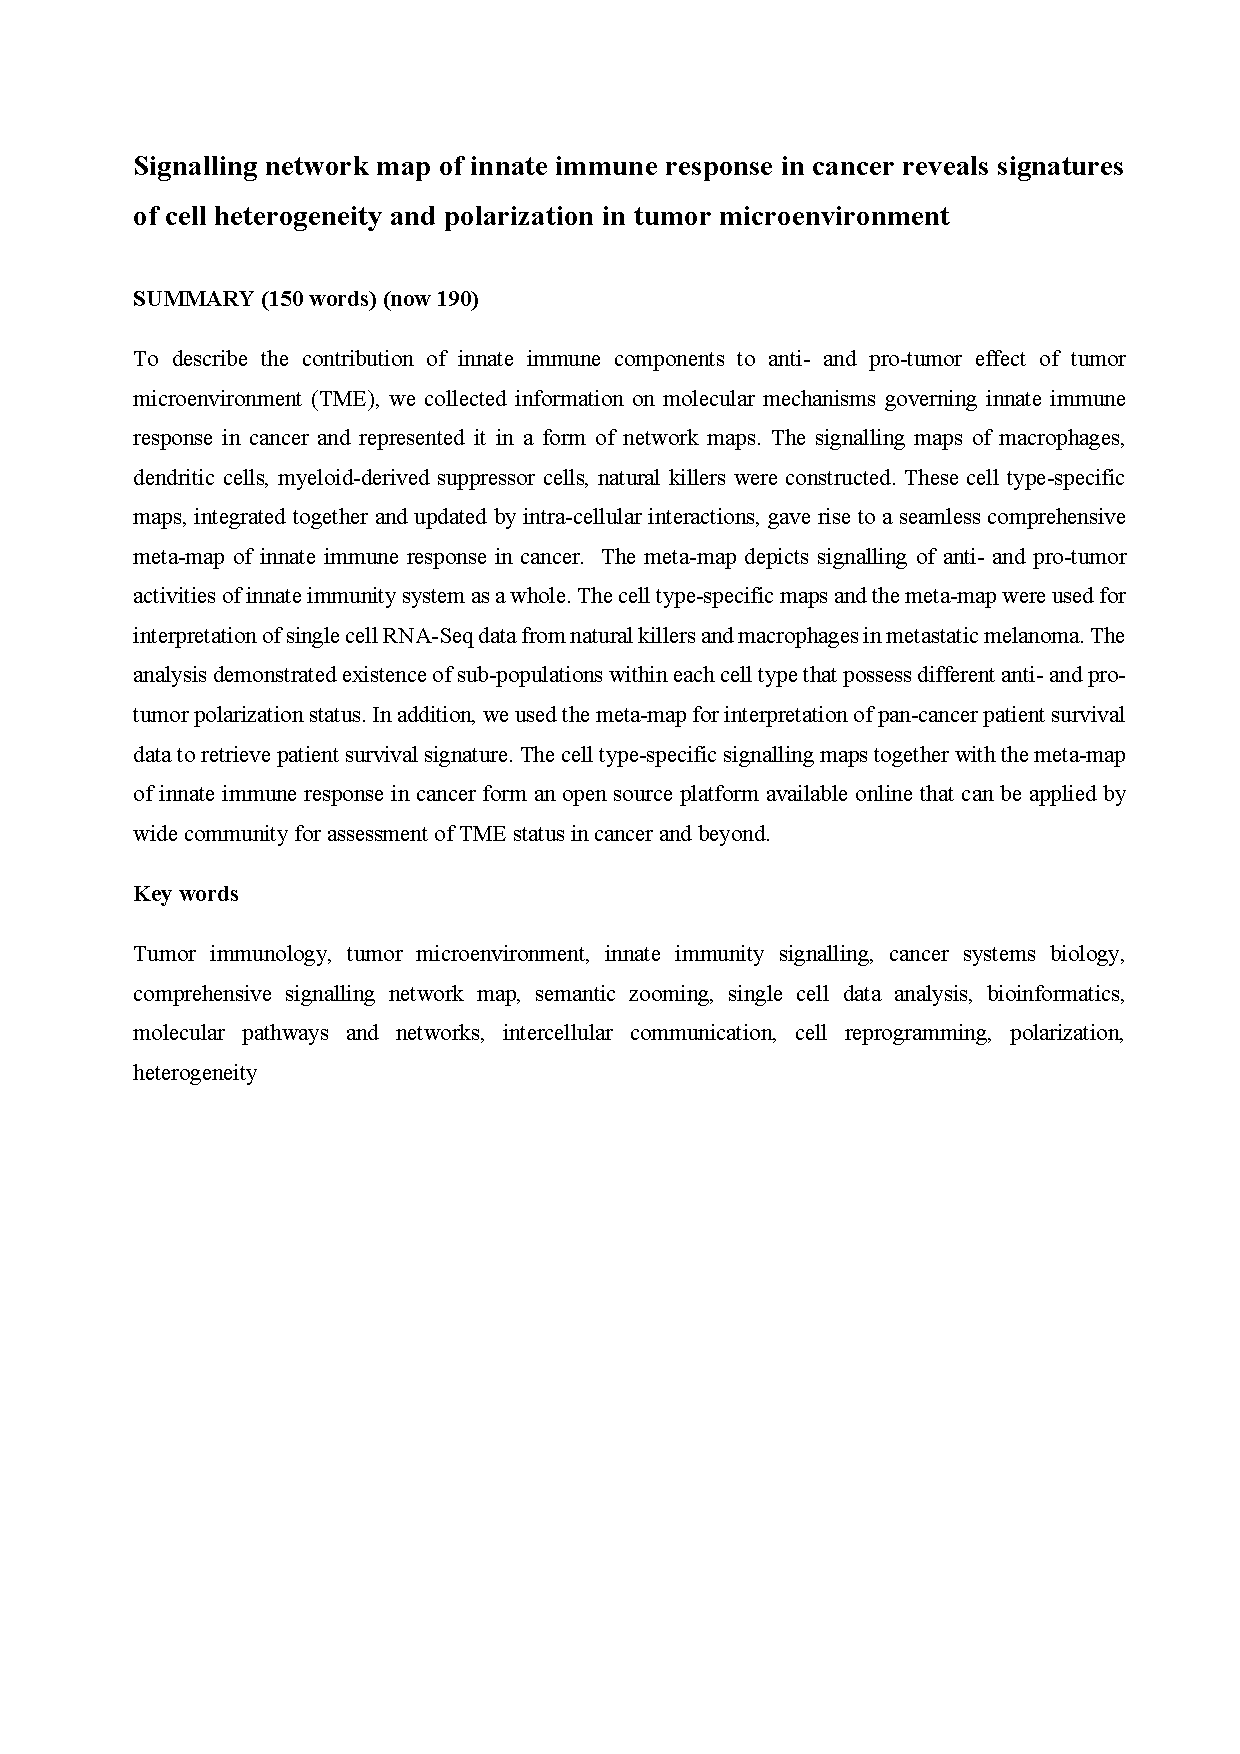
\includepdf[scale=1]{pdf-ext/ImmuneMap.pdf}

\hypertarget{conclusions}{%
\chapter{Conclusions and perspectives}\label{conclusions}}

\hypertarget{annexes}{%
\chapter*{Annexes}\label{annexes}}
\addcontentsline{toc}{chapter}{Annexes}

\emph{Note: This annexes will not be a part of final manuscript}

\hypertarget{phd-timeline-for-defence-before-the-end-of-october-2018}{%
\section*{PhD timeline for defence before the end of October
2018}\label{phd-timeline-for-defence-before-the-end-of-october-2018}}
\addcontentsline{toc}{section}{PhD timeline for defence before the end
of October 2018}

In order to defend before 31 October, I need to follow the guidelines of
the University.

\begin{itemize}
\tightlist
\item
  \textasciitilde{}29 June - officially submlit the jury proposal and a
  draft of the thesis to the university
\item
  \textasciitilde{}end of July - send manuscript to reviewers
\item
  24 Septemeber - 31 October - defend
\end{itemize}

\begin{figure}
\centering
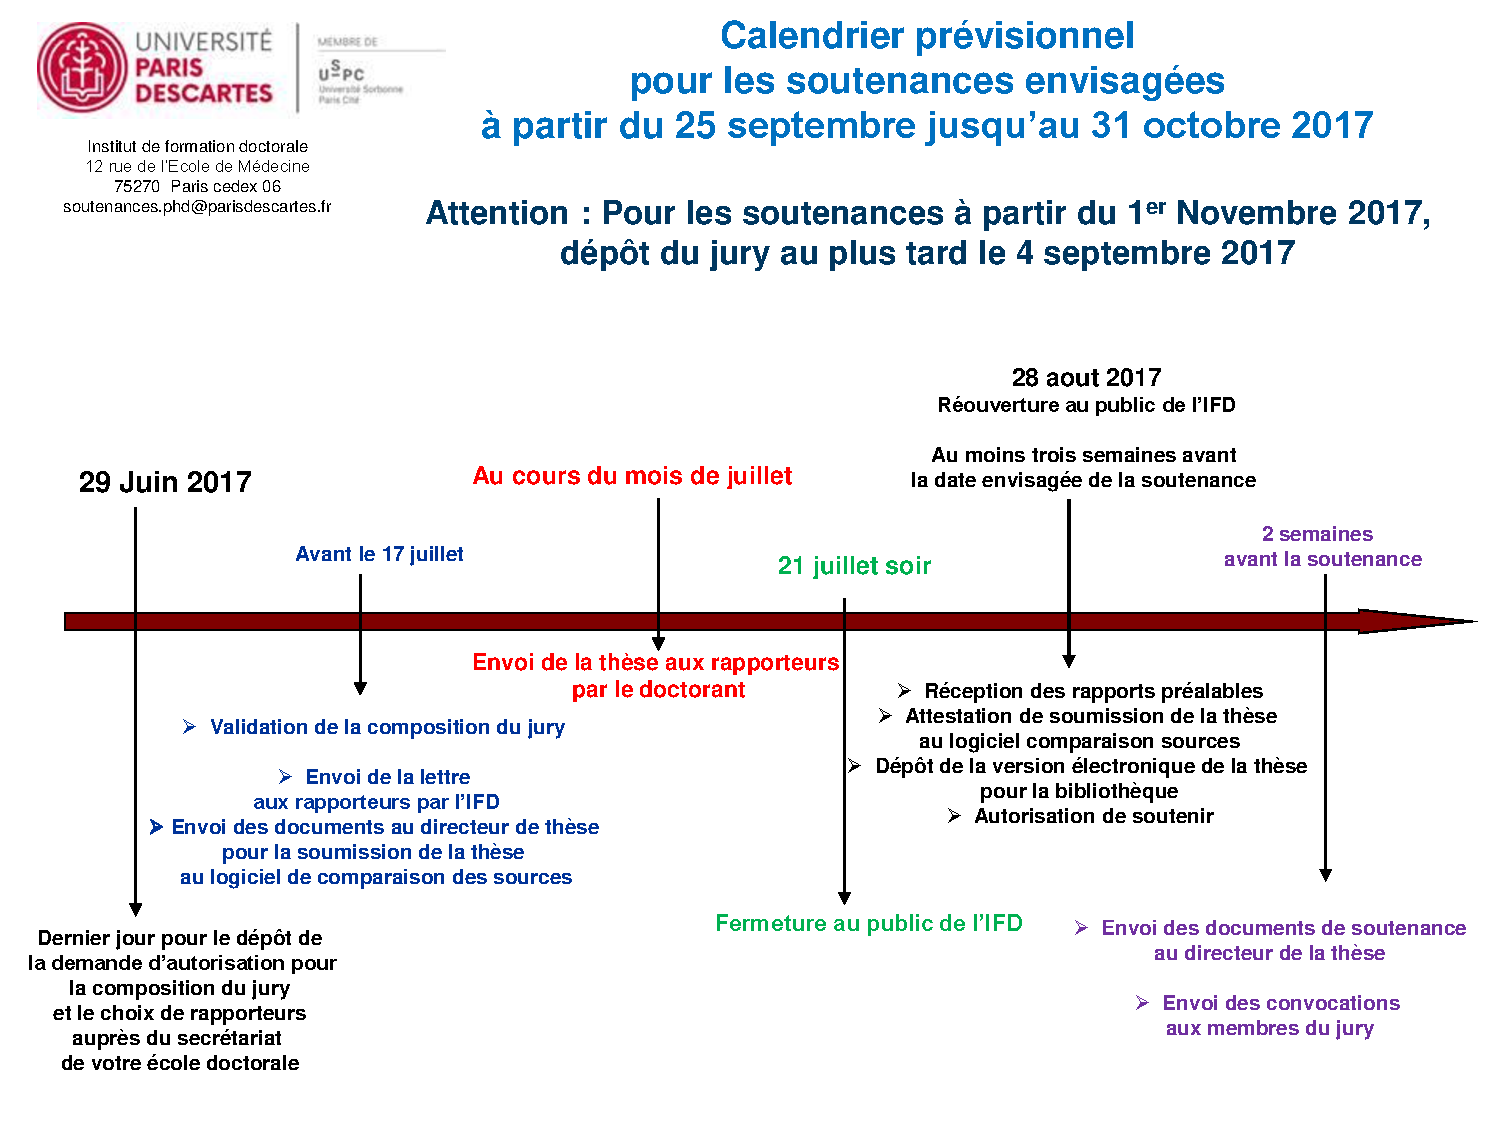
\includegraphics{figures-ext/An-timeline.pdf}
\caption{Timeline provided by University Paris Descartes for 2017}
\end{figure}

\hypertarget{thesis-writing}{%
\section*{Thesis writing}\label{thesis-writing}}
\addcontentsline{toc}{section}{Thesis writing}

This Report is written in
\href{https://github.com/rstudio/bookdown}{\emph{bookdown}}. I have
chosen this form as it can easily compile to \emph{LaTeX}, PDF, MS Word,
ebook and html. Optimally, the final manuscript will be also published
online in a form of an open source
\href{https://www.gitbook.com/about}{gitBook} and an ebook including
interactive figures and maybe even data demos. Another good reason for
using \href{https://github.com/rstudio/bookdown}{\emph{bookdown}} is its
simple syntax of markdown and natural integration of code snippets with
.Rmd. It reduces formatting time and give multiple outputs.

The template of for this thesis manuscript was adapted from \emph{LaTeX}
template provided by University Paris Descartes.

The format \emph{thesis by publication} will be considered for parts of
the thesis.

\newpage

\hypertarget{activity-report-2017}{%
\section*{Activity Report 2017}\label{activity-report-2017}}
\addcontentsline{toc}{section}{Activity Report 2017}

This documents list main achievements of 2017 including conference,
posters and publications list.

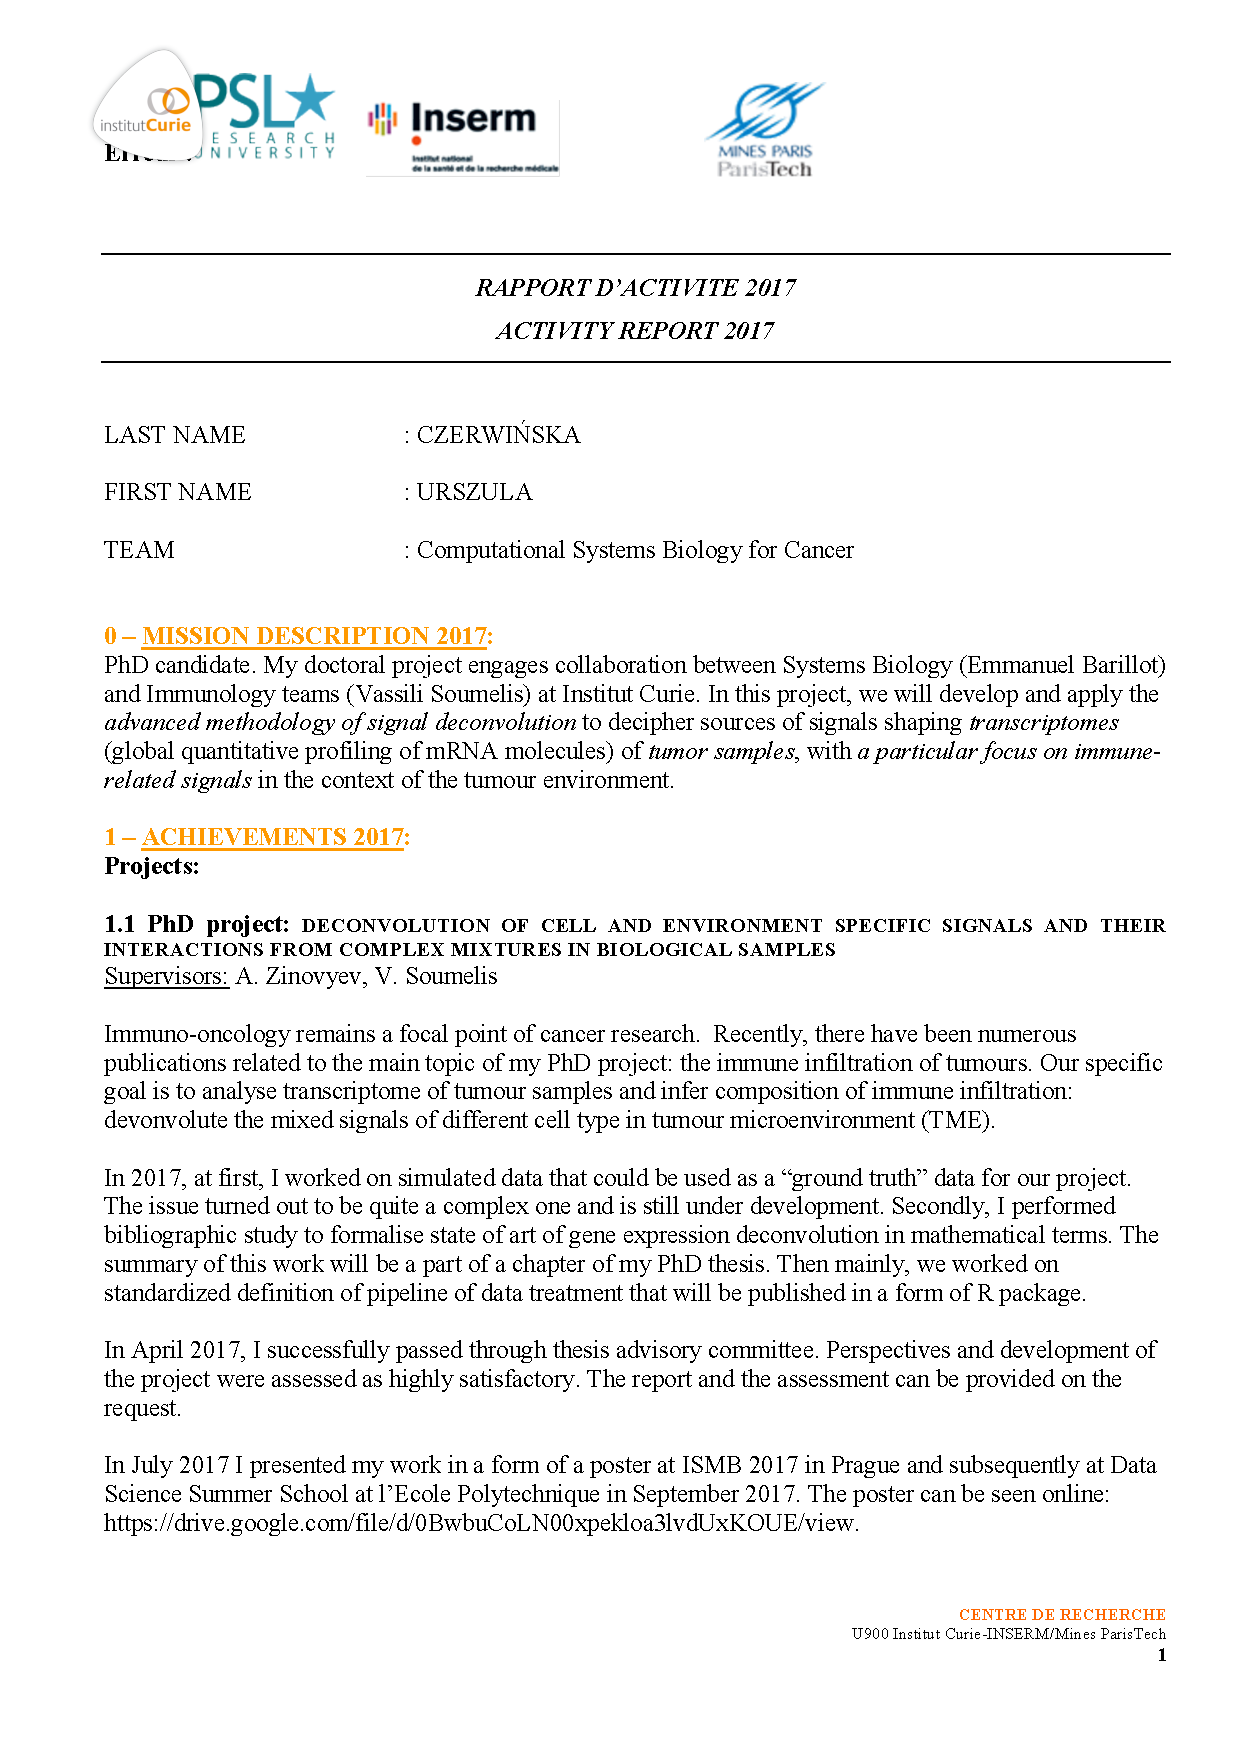
\includepdf[pages={1-}, scale=1]{pdf-ext/An-RA2017.pdf}

\bibliography{01-Intro.bib,packages.bib,UCzcite.bib}


\end{document}
